\documentclass[../main.tex]{subfiles}

\begin{document}

\setlength\parindent{0pt}

\subsection{Getting start}

Import \acode{tikz} pacakage by \acode{\\usepackage{tikz}}, and use it in tex:

\begin{lstlisting}
  \begin{tikzpicture}
    <code goes here>
  \end{tikzpicture}
\end{lstlisting}

\subsubsection{Basic shapes}

Note: finish the satement by closing it with a semicolon.

\bigskip

A strait line:

\begin{center}
  \begin{tikzpicture}
    \draw (0,0) -- (4,0);
  \end{tikzpicture}
\end{center}

Make a square by \acode{\\draw (0,0) -- (4,0) -- (4,4) -- (0,4) -- (0,4) -- cycle}:

\begin{center}
  \begin{tikzpicture}
    \draw (0,0) -- (4,0) -- (4,4) -- (0,4) -- (0,4) -- cycle;
  \end{tikzpicture}
\end{center}

Or simplified \acode{\\draw (0,0) rectangle (4,4);}:

\begin{center}
  \begin{tikzpicture}
    \draw (0,0) rectangle (4,4);
  \end{tikzpicture}
\end{center}

A parabola \acode{\\draw (0,0) parabola (4,4);}:

\begin{center}
  \begin{tikzpicture}
    \draw (0,0) parabola (4,4);
  \end{tikzpicture}
\end{center}

Add a curved line by using \textit{control points}, \acode{\\draw (0,0) .. controls (0,4) and (4,0) .. (4,4);}:

\begin{center}
  \begin{tikzpicture}
    \draw (0,0) .. controls (0,4) and (4,0) .. (4,4);
  \end{tikzpicture}
\end{center}

A circle by \acode{\\draw (2,2) circle (3cm);}:

\begin{center}
  \begin{tikzpicture}
    \draw (2,2) circle (3cm);
  \end{tikzpicture}
\end{center}

An ellipse by \acode{\\draw (2,2) ellipse (3cm and 1cm);}:

\begin{center}
  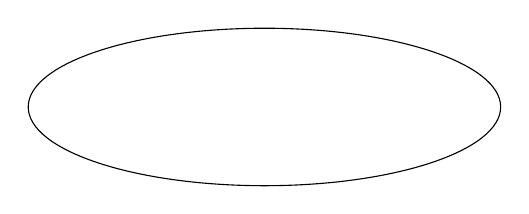
\begin{tikzpicture}
    \draw (2,2) ellipse (3cm and 1cm);
  \end{tikzpicture}
\end{center}

An arc by \acode{\\draw (3,0) arc (0:75:3cm);}:

\begin{center}
  \begin{tikzpicture}
    \draw (3,0) arc (0:75:3cm);
  \end{tikzpicture}
\end{center}

A costomised circle by \acode{\\draw[red,thick,dashed] (2,2) circle (3cm);}:

\begin{center}
  \begin{tikzpicture}
    \draw[red,thick,dashed] (2,2) circle (3cm);
  \end{tikzpicture}
\end{center}

\subsubsection{Grids}

A grid by \acode{\\draw[step=1cm,gray,very thin] (-2,-2) grid (6,6);}:

\begin{center}
  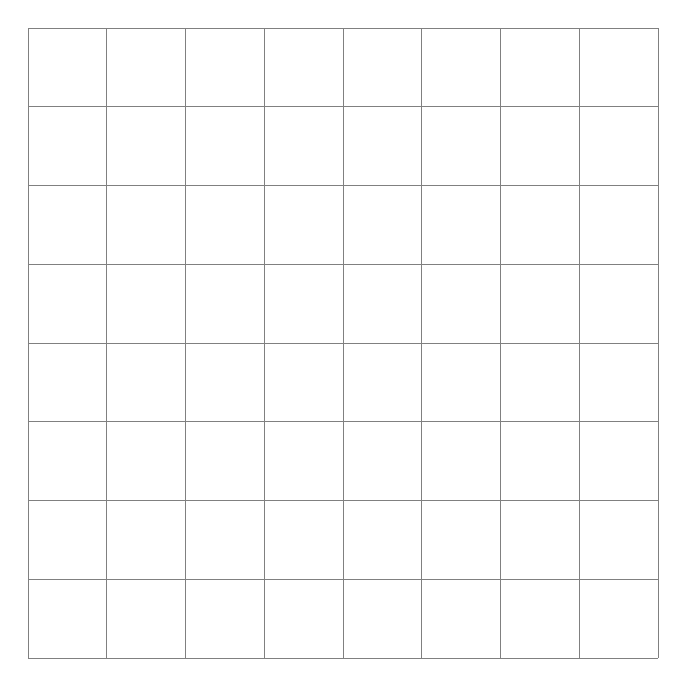
\begin{tikzpicture}
    \draw[step=1cm,gray,very thin] (-2,-2) grid (6,6);
  \end{tikzpicture}
\end{center}

A removed outer lines grid \acode{\\draw[step=1cm,gray,very thin] (-1.9,-1.9) grid (5.9,5.9);}:

\begin{center}
  \begin{tikzpicture}
    \draw[step=1cm,gray,very thin] (-1.9,-1.9) grid (5.9,5.9);
  \end{tikzpicture}
\end{center}

A color filled rectangle by \acode{\\fill[blue!40!white] (0,0) rectangle (4,4);}

\begin{center}
  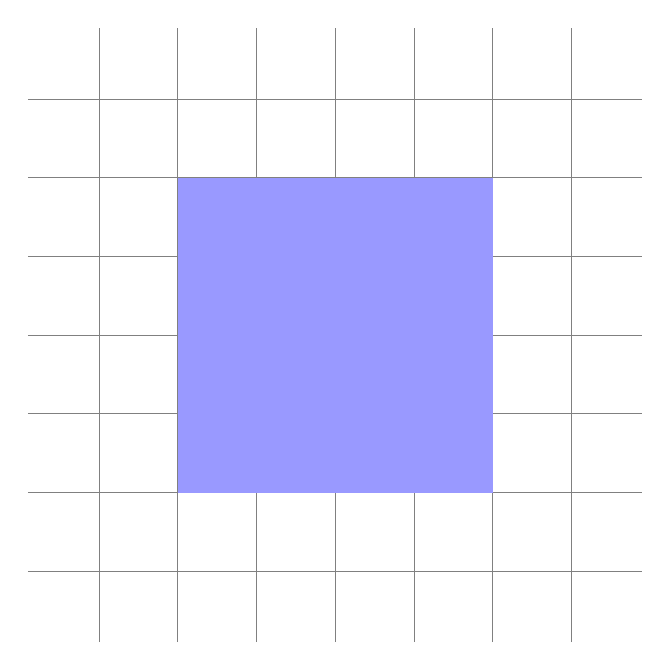
\begin{tikzpicture}
    \draw[step=1cm,gray,very thin] (-1.9,-1.9) grid (5.9,5.9);
    \fill[blue!40!white] (0,0) rectangle (4,4);
  \end{tikzpicture}
\end{center}

and a border added \acode{\\filldraw[fill=blue!40!white, draw=black] (0,0) rectangle (4,4);}:

\begin{center}
  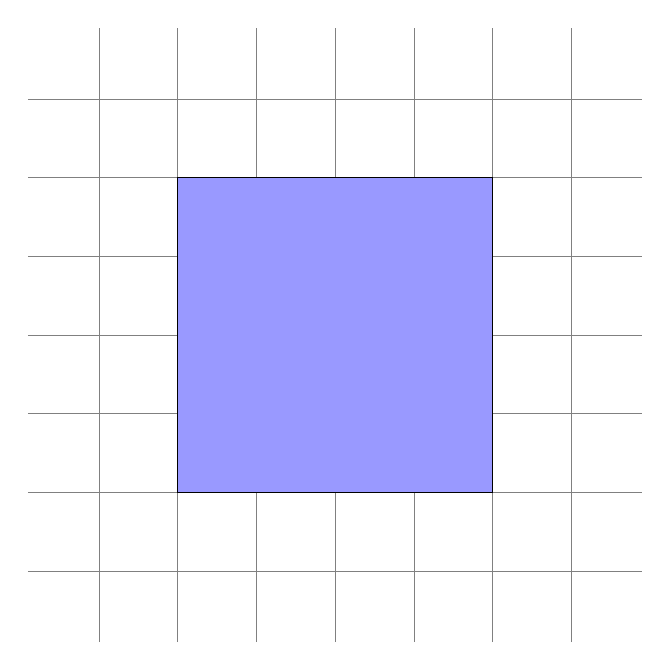
\begin{tikzpicture}
    \draw[step=1cm,gray,very thin] (-1.9,-1.9) grid (5.9,5.9);
    \filldraw[fill=blue!40!white, draw=black] (0,0) rectangle (4,4);
  \end{tikzpicture}
\end{center}

and shading \acode{\\shade[left color=blue,right color=red] (0,0) rectangle (4,4);}

\begin{center}
  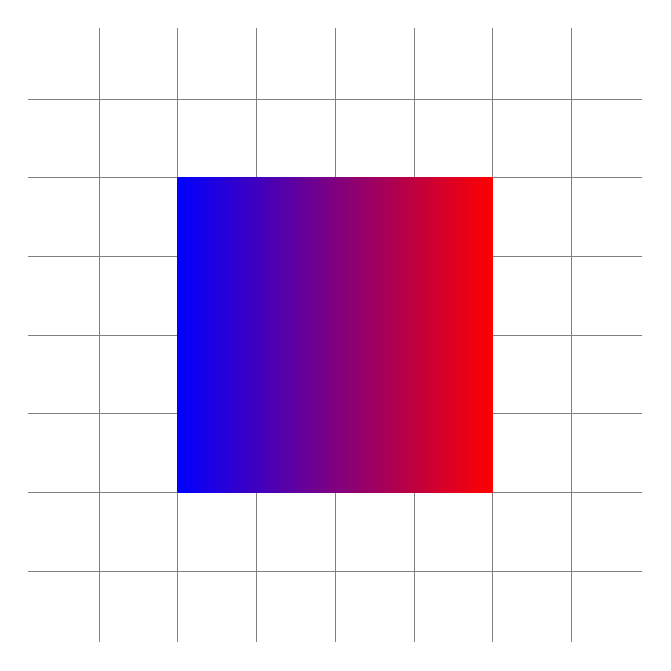
\begin{tikzpicture}
    \draw[step=1cm,gray,very thin] (-1.9,-1.9) grid (5.9,5.9);
    \shade[left color=blue,right color=red] (0,0) rectangle (4,4);
  \end{tikzpicture}
\end{center}

and shading in the vertical direction \acode{\\shade[top color=blue,bottom color=red] (0,0) rectangle (4,4);}

\begin{center}
  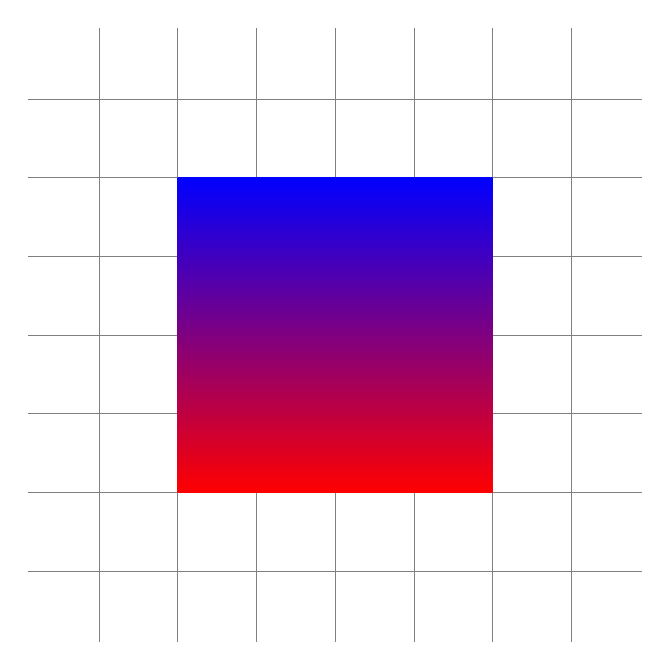
\begin{tikzpicture}
    \draw[step=1cm,gray,very thin] (-1.9,-1.9) grid (5.9,5.9);
    \shade[top color=blue,bottom color=red] (0,0) rectangle (4,4);
  \end{tikzpicture}
\end{center}

radiation \acode{\\shade[inner color=blue,outer color=red] (0,0) rectangle (4,4);}

\begin{center}
  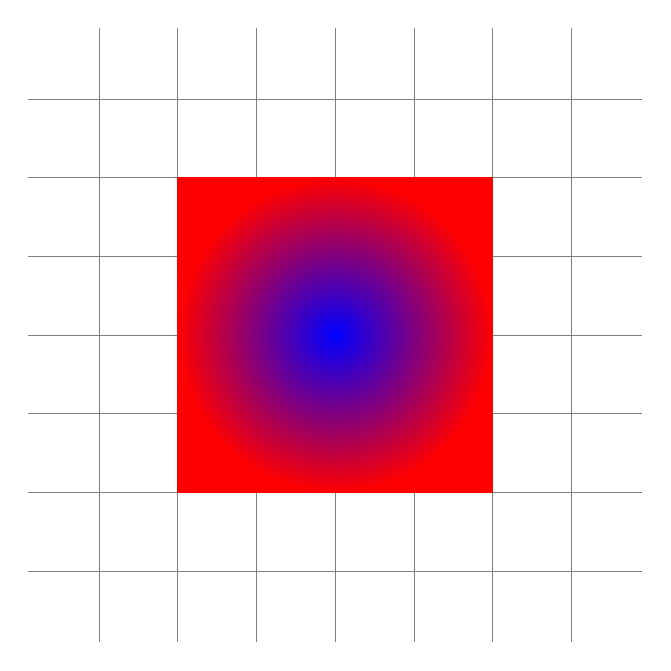
\begin{tikzpicture}
    \draw[step=1cm,gray,very thin] (-1.9,-1.9) grid (5.9,5.9);
    \shade[inner color=blue,outer color=red] (0,0) rectangle (4,4);
  \end{tikzpicture}
\end{center}

add border \acode{\\shadedraw[inner color=blue,outer color=red, draw=black] (0,0) rectangle (4,4);}

\begin{center}
  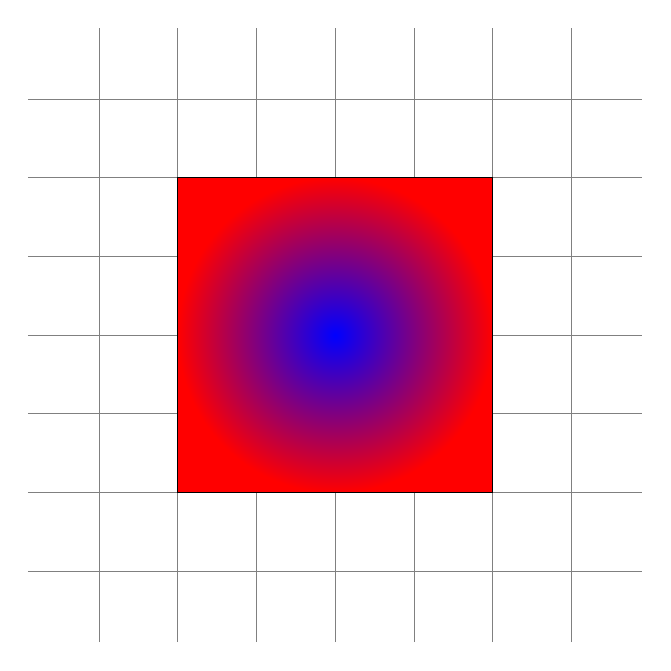
\begin{tikzpicture}
    \draw[step=1cm,gray,very thin] (-1.9,-1.9) grid (5.9,5.9);
    \shadedraw[inner color=blue,outer color=red, draw=black] (0,0) rectangle (4,4);
  \end{tikzpicture}
\end{center}

\subsubsection{Axes}

Two vectors \acode{\\draw[thick,->] (0,0) -- (4.5,0);}:

\begin{center}
  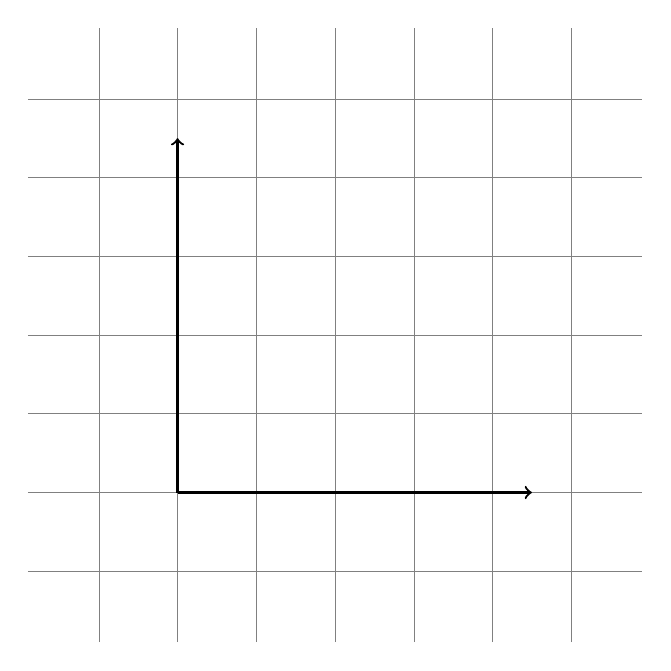
\begin{tikzpicture}
    \draw[step=1cm,gray,very thin] (-1.9,-1.9) grid (5.9,5.9);
    \draw[thick,->] (0,0) -- (4.5,0);
    \draw[thick,->] (0,0) -- (0,4.5);
  \end{tikzpicture}
\end{center}

add ticks and numbers:

\begin{lstlisting}
  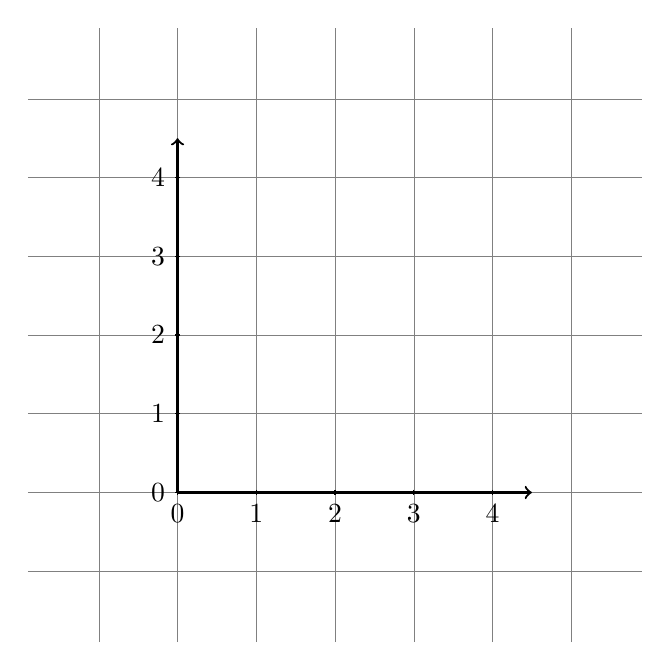
\begin{tikzpicture}
    \draw[step=1cm,gray,very thin] (-1.9,-1.9) grid (5.9,5.9);
    \draw[thick,->] (0,0) -- (4.5,0);
    \draw[thick,->] (0,0) -- (0,4.5);
    \foreach \x in {0,1,2,3,4}
    \draw (\x cm,1pt) -- (\x cm,-1pt) node[anchor=north] {$\x$};
    \foreach \y in {0,1,2,3,4}
    \draw (1pt,\y cm) -- (-1pt,\y cm) node[anchor=east] {$\y$};
  \end{tikzpicture}
\end{lstlisting}

\begin{center}
  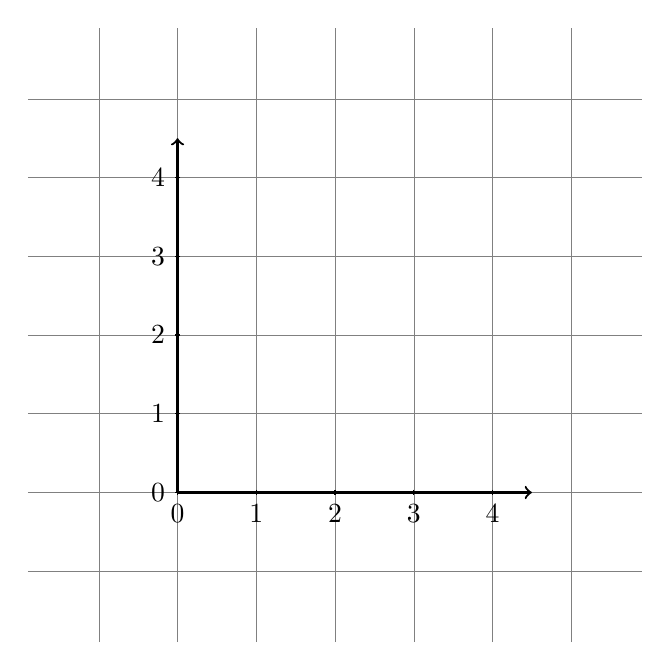
\begin{tikzpicture}
    \draw[step=1cm,gray,very thin] (-1.9,-1.9) grid (5.9,5.9);
    \draw[thick,->] (0,0) -- (4.5,0);
    \draw[thick,->] (0,0) -- (0,4.5);
    \foreach \x in {0,1,2,3,4}
    \draw (\x cm,1pt) -- (\x cm,-1pt) node[anchor=north] {$\x$};
    \foreach \y in {0,1,2,3,4}
    \draw (1pt,\y cm) -- (-1pt,\y cm) node[anchor=east] {$\y$};
  \end{tikzpicture}
\end{center}

\end{document}
